% Elekes's point-line configuration for A={1,2,3,4} (generated by a script).
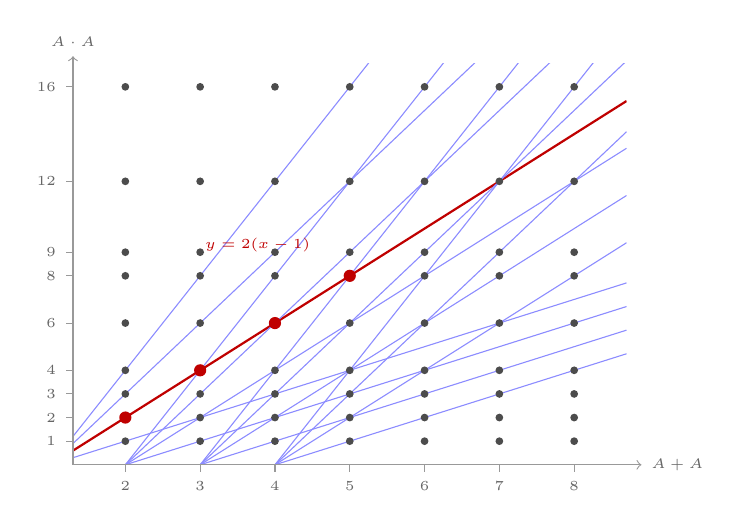
\begin{tikzpicture}[x=0.95cm,y=0.30cm]
\begin{scope}
\clip (1.3,0) rectangle (8.7,17);
\draw[blue!45,thin] (1.30,0.30)--(8.70,7.70);
\draw[blue!45,thin] (1.30,-0.70)--(8.70,6.70);
\draw[blue!45,thin] (1.30,-1.70)--(8.70,5.70);
\draw[blue!45,thin] (1.30,-2.70)--(8.70,4.70);
\draw[red!75!black,thick] (1.30,0.60)--(8.70,15.40);
\draw[blue!45,thin] (1.30,-1.40)--(8.70,13.40);
\draw[blue!45,thin] (1.30,-3.40)--(8.70,11.40);
\draw[blue!45,thin] (1.30,-5.40)--(8.70,9.40);
\draw[blue!45,thin] (1.30,0.90)--(8.70,23.10);
\draw[blue!45,thin] (1.30,-2.10)--(8.70,20.10);
\draw[blue!45,thin] (1.30,-5.10)--(8.70,17.10);
\draw[blue!45,thin] (1.30,-8.10)--(8.70,14.10);
\draw[blue!45,thin] (1.30,1.20)--(8.70,30.80);
\draw[blue!45,thin] (1.30,-2.80)--(8.70,26.80);
\draw[blue!45,thin] (1.30,-6.80)--(8.70,22.80);
\draw[blue!45,thin] (1.30,-10.80)--(8.70,18.80);
\end{scope}
\draw[black!40,->] (1.3,0)--(8.9,0) node[right,font=\tiny,black!60]{$A+A$};
\draw[black!40,->] (1.3,0)--(1.3,17.3) node[above,font=\tiny,black!60]{$A\cdot A$};
\draw[black!40] (2,0)--(2,-0.3) node[below,font=\tiny,black!60]{$2$};
\draw[black!40] (3,0)--(3,-0.3) node[below,font=\tiny,black!60]{$3$};
\draw[black!40] (4,0)--(4,-0.3) node[below,font=\tiny,black!60]{$4$};
\draw[black!40] (5,0)--(5,-0.3) node[below,font=\tiny,black!60]{$5$};
\draw[black!40] (6,0)--(6,-0.3) node[below,font=\tiny,black!60]{$6$};
\draw[black!40] (7,0)--(7,-0.3) node[below,font=\tiny,black!60]{$7$};
\draw[black!40] (8,0)--(8,-0.3) node[below,font=\tiny,black!60]{$8$};
\draw[black!40] (1.3,1)--(1.2,1) node[left,font=\tiny,black!60]{$1$};
\draw[black!40] (1.3,2)--(1.2,2) node[left,font=\tiny,black!60]{$2$};
\draw[black!40] (1.3,3)--(1.2,3) node[left,font=\tiny,black!60]{$3$};
\draw[black!40] (1.3,4)--(1.2,4) node[left,font=\tiny,black!60]{$4$};
\draw[black!40] (1.3,6)--(1.2,6) node[left,font=\tiny,black!60]{$6$};
\draw[black!40] (1.3,8)--(1.2,8) node[left,font=\tiny,black!60]{$8$};
\draw[black!40] (1.3,9)--(1.2,9) node[left,font=\tiny,black!60]{$9$};
\draw[black!40] (1.3,12)--(1.2,12) node[left,font=\tiny,black!60]{$12$};
\draw[black!40] (1.3,16)--(1.2,16) node[left,font=\tiny,black!60]{$16$};
\fill[black!70] (2,1) circle (1.4pt);
\fill[red!75!black] (2,2) circle (2.2pt);
\fill[black!70] (2,3) circle (1.4pt);
\fill[black!70] (2,4) circle (1.4pt);
\fill[black!70] (2,6) circle (1.4pt);
\fill[black!70] (2,8) circle (1.4pt);
\fill[black!70] (2,9) circle (1.4pt);
\fill[black!70] (2,12) circle (1.4pt);
\fill[black!70] (2,16) circle (1.4pt);
\fill[black!70] (3,1) circle (1.4pt);
\fill[black!70] (3,2) circle (1.4pt);
\fill[black!70] (3,3) circle (1.4pt);
\fill[red!75!black] (3,4) circle (2.2pt);
\fill[black!70] (3,6) circle (1.4pt);
\fill[black!70] (3,8) circle (1.4pt);
\fill[black!70] (3,9) circle (1.4pt);
\fill[black!70] (3,12) circle (1.4pt);
\fill[black!70] (3,16) circle (1.4pt);
\fill[black!70] (4,1) circle (1.4pt);
\fill[black!70] (4,2) circle (1.4pt);
\fill[black!70] (4,3) circle (1.4pt);
\fill[black!70] (4,4) circle (1.4pt);
\fill[red!75!black] (4,6) circle (2.2pt);
\fill[black!70] (4,8) circle (1.4pt);
\fill[black!70] (4,9) circle (1.4pt);
\fill[black!70] (4,12) circle (1.4pt);
\fill[black!70] (4,16) circle (1.4pt);
\fill[black!70] (5,1) circle (1.4pt);
\fill[black!70] (5,2) circle (1.4pt);
\fill[black!70] (5,3) circle (1.4pt);
\fill[black!70] (5,4) circle (1.4pt);
\fill[black!70] (5,6) circle (1.4pt);
\fill[red!75!black] (5,8) circle (2.2pt);
\fill[black!70] (5,9) circle (1.4pt);
\fill[black!70] (5,12) circle (1.4pt);
\fill[black!70] (5,16) circle (1.4pt);
\fill[black!70] (6,1) circle (1.4pt);
\fill[black!70] (6,2) circle (1.4pt);
\fill[black!70] (6,3) circle (1.4pt);
\fill[black!70] (6,4) circle (1.4pt);
\fill[black!70] (6,6) circle (1.4pt);
\fill[black!70] (6,8) circle (1.4pt);
\fill[black!70] (6,9) circle (1.4pt);
\fill[black!70] (6,12) circle (1.4pt);
\fill[black!70] (6,16) circle (1.4pt);
\fill[black!70] (7,1) circle (1.4pt);
\fill[black!70] (7,2) circle (1.4pt);
\fill[black!70] (7,3) circle (1.4pt);
\fill[black!70] (7,4) circle (1.4pt);
\fill[black!70] (7,6) circle (1.4pt);
\fill[black!70] (7,8) circle (1.4pt);
\fill[black!70] (7,9) circle (1.4pt);
\fill[black!70] (7,12) circle (1.4pt);
\fill[black!70] (7,16) circle (1.4pt);
\fill[black!70] (8,1) circle (1.4pt);
\fill[black!70] (8,2) circle (1.4pt);
\fill[black!70] (8,3) circle (1.4pt);
\fill[black!70] (8,4) circle (1.4pt);
\fill[black!70] (8,6) circle (1.4pt);
\fill[black!70] (8,8) circle (1.4pt);
\fill[black!70] (8,9) circle (1.4pt);
\fill[black!70] (8,12) circle (1.4pt);
\fill[black!70] (8,16) circle (1.4pt);
\node[font=\tiny,red!75!black,above left] at (4.6,8.6) {$y=2(x-1)$};
\end{tikzpicture}
